\begin{frame}[t]
    \frametitle{Results: Canonical refining}
    \framesubtitle{Discovering \textit{de-novo} miRNAs}
    \begin{figure}[h!]
        \centering
        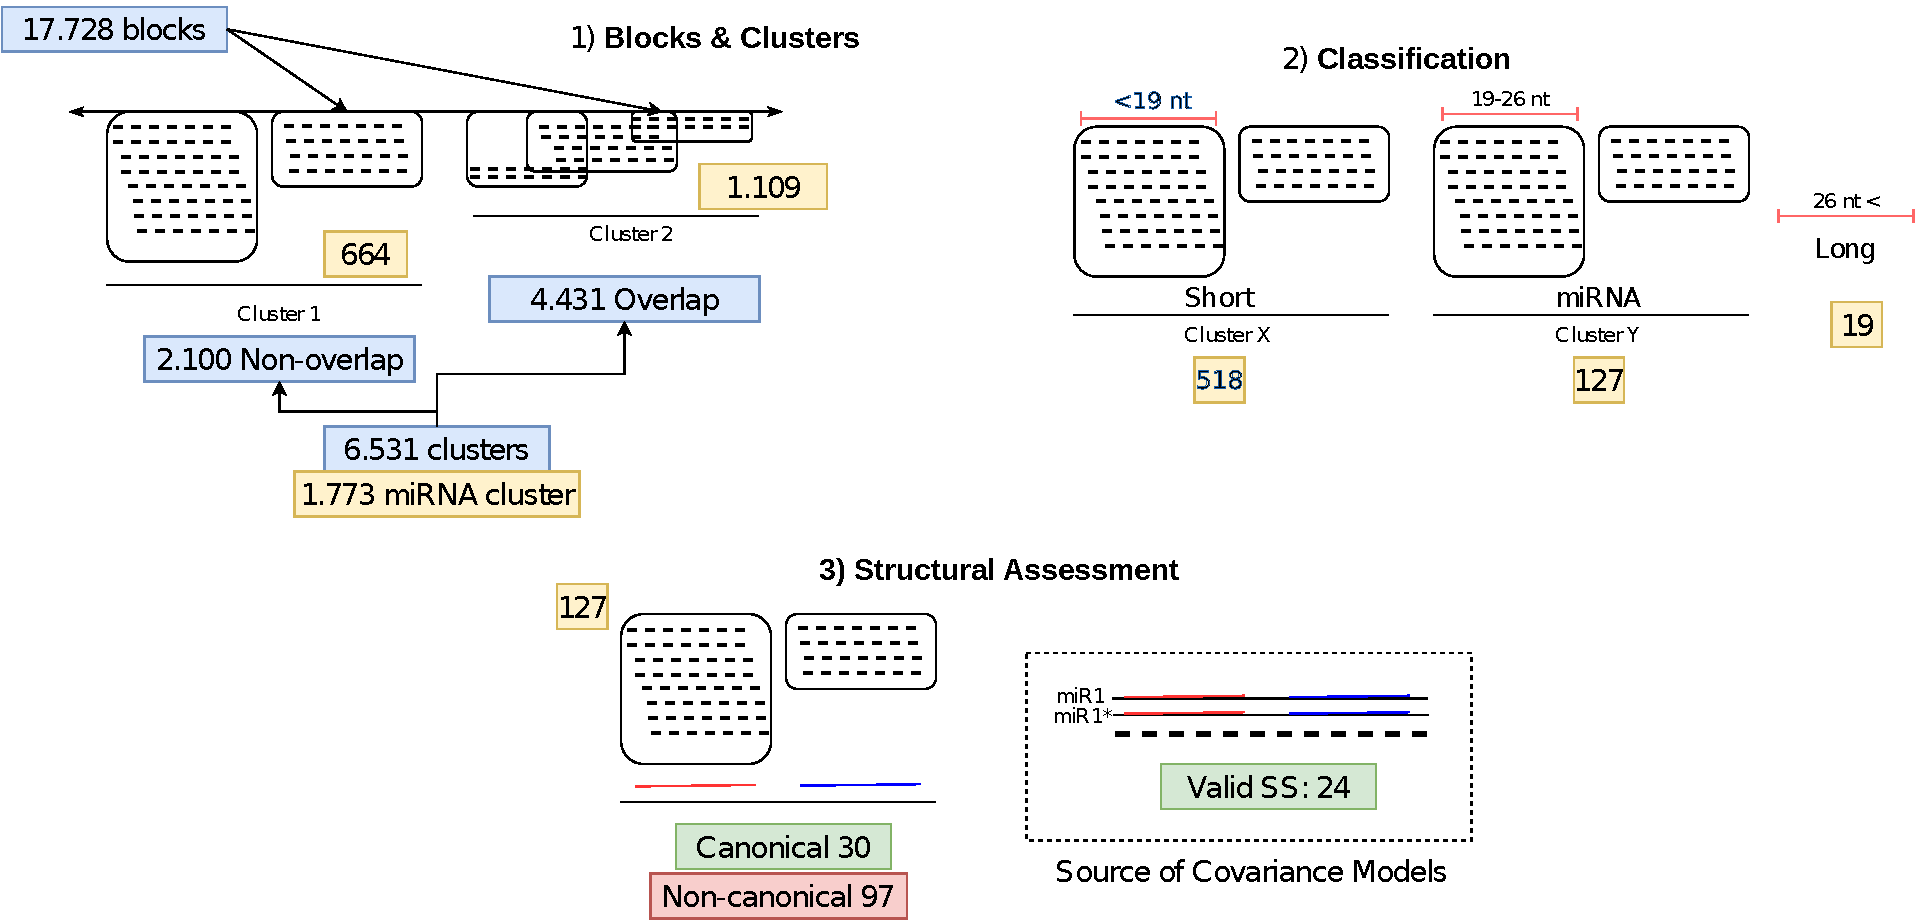
\includegraphics[width=\linewidth]{Figures/results_workflowALL}\label{fig:workflow} %
    \end{figure}
    \begin{itemize}
        \item Only $3.6$ \% potential candidates detected as \textit{canonical} miRNAs.
        \item Expression of potential piwi-RNAs covers most of the candidates ($\sim 77.4$\%)
    \end{itemize}
\end{frame}

\begin{frame}[t]
    % Take the most expressed candidates from the 24 ones and show one comparison.
    \frametitle{Results: Previous example}
    Finding canonical de-novo families.
    \begin{figure}[h!]
        \centering
        \includegraphics<1>[width=\linewidth]{Figures/chr7_cluster} %
    \end{figure}
     Two additional candidates covered by de-novo expression patterns $:($
     \begin{itemize}
         \item Why those families are not covered? 
     \end{itemize}
\end{frame}


\begin{frame}[t]
    % Take the most expressed candidates from the 24 ones and show one comparison.
    \frametitle{Results: miRNAs on Ascidians}
    \begin{itemize}
        \item \textit{C.\ robusta} annotations: $351$ loci
        \item With Fam.: $18.5$\% / No Fam: $81.5$\%.
        \item $13\times$ than sister specie: \textit{Ciona savignyi}
        \item Higher loci number than coelacanth and lancelet (!).
    \end{itemize}
    % Make a plot of the miRBase validation from table in:
    %/scr/k70san/bogota_unal/tunicata_micro_Evolution/Code/CountingValidatedFinal/Code
\end{frame}


\begin{frame}[t]
    % Take the most expressed candidates from the 24 ones and show one comparison.
    \frametitle{Results: Previous example}
    Finding canonical de-novo families.
    \begin{figure}[h!]
        \centering
        \includegraphics<1>[width=\linewidth]{Figures/evaluation_annotation_mirbase1} %
        \includegraphics<2>[width=\linewidth]{Figures/evaluation_annotation_mirbase2} %
    \end{figure}
     \begin{itemize}[<+->]
         \item Canonical miRNAs on cluster chr7 covered $~16$\% of cluster.
         \item Reasons: Position of mature sequences, loop regions, structural constrains.
     \end{itemize}
\end{frame}

\begin{frame}[t]
    \frametitle{Results: Iteration $1$}
    \framesubtitle{Discovering \textit{de-novo} miRNAs}
    \begin{itemize}
        \item Starting point: $24$ CMs from \textit{C.\ robusta}.
        \item First target specie: \textit{Ciona savignyi}.
    \end{itemize}
\end{frame}
